% ------------------------------------------------------------------------ %
% !TEX encoding = UTF-8 Unicode
% !TEX TS-program = pdflatex
% !TEX root = ../Tesi.tex
% !TeX spellcheck = en_US
% ------------------------------------------------------------------------ %
%
% ------------------------------------------------------------------------ %
% 	CONCLUSIONI
% ------------------------------------------------------------------------ %
%
\chapter{Case Study}
%
\label{cap:proofofconcept}
%
% ------------------------------------------------------------------------%
In this chapter I will describe the real implementation of the system, which is the real solution of the problem faced by this thesis work: how it is possible to extend a mobile operating system, in this case Android, with distributed OS functionalities.\\
This chapter is mainly composed of three parts: the first one is a generic information
section in which the proof of concept is explained in terms of technologies
used, requirements to meet, goals and various technicalities. The second one
is the report of the implementation and development of the application, with
choices and descriptions of what has been done. The third part is a working demo of the
just described system, with live working test cases. It contains screenshots of the
application while it is running and a complete description to explain each case
step by step.
\section{Design Choices}
\subsection{Application Description}
As already specified in the previous chapter my system has been implemented as a standard Android application, which can be installed on any Android device starting from the API level 19, Android 4.4 KitKat. The final APK package contains all the files needed for the system installation, and, once installed, the application performs the extension of the Android OS giving to it distributed functionalities. I will use the complete API described in \ref{API} to implement a background working middleware to distribute implicit intent in a LAN to any Android device with the service installed. In this way every time one of the device, having the \textit{Liquid Android APK}
installed, triggers an implicit intent, my application could intercept and send it to any other device to be resolved and executed. The idea of this prototype is to prove that what I have stated, providing the theoretical solution, can work with a real configuration of Android devices in any LAN. Doing this, the thesis work is somehow \textit{"proved"}: my communication language, defined with a JSON file, is concretely usable and working, not to worry the users about the kind of implicit intent they need to execute in one of the devices in the network. The translation process does not represent an issue for my application, because I have developed an automatic intent translator using the correct syntax proposed by me. I will not develop clients for third party systems, even if I stated that it would be possible, especially in Java environments, but I will implement a simple Android application client, generating some standard implicit intent to perform some test with my system.
\subsection{Requirements}
In this small subsection I want to provide a full list of requirements my application must meet. In order to be considered a solution of the given problem, it must fulfill the constrains listed in \ref{problemconstraints} and also comply with functional and non functional requirements.
\subsubsection{Functional Requirements}
Functional requirements are, indeed, the main functionalities the systems must have in order to properly work to perform desired task.\\
The following lists summarize the main features of the system, so as to ensure a quick reference while reading this document:
\begin{itemize}
	\item \textbf{FR1}: listen to implicit intents.\\My application should declare itself, in the android manifest, as a multipurpose application which can be used to resolve, basically, any kind of implicit intents, in order to be selected by the Android OS whenever an intent resolution process is triggered.
	\item \textbf{FR2}: JSON to Intent, and Intent to JSON, conversion.\\ My application must be able to perform the conversion using the JSON syntax i have explained in \ref{syntax}.
	\item \textbf{FR3}: forward implicit intents.\\ My application must be able to forward any of the implicit intent it can listen, to other LAN connected devices with the \textit{Liquid Android APK} installed.
	\item \textbf{FR4}: receive and execute intents.\\ My application must be able to receive in any moment implicit intents, as JSON-Intent object, and then, let the OS resolve and execute them with its standard mechanisms.
\end{itemize}
\subsubsection{Non-Functional Requirements}
Non-functional requirements are important properties that my
system must have in order to guarantee full functionalities. They are not specific
for my problem but, they are general requirements a system needs to be considered complete. It is quite clear how a system can use my language but if it takes 15 minutes to perform a translation or to deliver a message it is completely useless.\\
Non-functional requirements in this way complete my system, they are mainly:
\begin{itemize}
	\item \textit{Portability}: to have my application used by the largest number of users
	possible, so i have made the choice to use Android API level 19, to allow the installation of my system to, more or less, the 84\% of Android devices currently active.
	\item \textit{Stability}: system must be always available, and able to offer all its services. For example I should avoid possible system crashes during the delivery of a message from a device to another. In addition, data must be durable and not lost for any reasons.
	\item \textit{Availability}: the services must be always accessible in time. In case of failures it is possible for the user to manually restart it to be again usable.
	\item \textit{Reliability}: since data are shared among devices, reliability is essential. Users can base their actions on other users’ actions and on the status of the devices. Moreover, I assume that the memory where data are stored is stable.
	\item \textit{Efficiency}: within software development framework, efficiency means
	using as few resources as possible. Thus, the system will provide data
	structures and algorithms aimed to maximize efficiency. I will also try to
	use well known patterns reusing as many pieces of code as possible, taking
	care of avoiding any anti-patterns.
	\item \textit{Extensibility}: my application must provide a design where future updates
	are possible. It will be developed in such a way that the addition of new
	functionalities will not require radical changes to the internal structure and
	data flow.
	\item \textit{Maintainability}: also modifications to a code that already exists have to be
	taken into account. For this reason the code must be easily readable and
	fully commented.
	\item \textit{Security}: Using a networking service security is always required. The fact that
	the system will be available only on LANs is the first step in this direction.
\end{itemize}
\subsection{Used Technologies}
This other subsection is an overview of the tools I have used to develop the
Android application.\\
Android applications are written using Java code and any API level of the Android framework. The \textit{Liquid Android APK} is been developed by using standard Android development tools and libraries without the need to rely on any third party API library. In particular I decided to make these choices.
\begin{itemize}
	\item \textit{Android API level 19}, as already explained several times I want that my system can be installed on the largest number of devices, so it is a compromise between the great innovation introduced starting from this API level, and the number of devices which can execute API level 19 apps.
	\item \textit{Android NSD library}, it is a standard Android library I am using to register, discover and resolve my network service. It is an implementation of Zeroconf and it is compatible with other implementation such as Apple's bonjour.
	\item \textit{Standard Java libraries}, I decided to use only libraries included in standard Java development kit distribution, the most important are :
	\begin{itemize}
		\item \textit{org.json}, used to manage the JSON file, which are the messages exchanged by the devices using my application;
		\item \textit{java.net}, containing the classes which are useful to implement the socket network communication.
	\end{itemize}	
\end{itemize}
Technically, I used an IDE to help in development, in particular AndroidStrudio based on IntelliJ IDEA, a
modern solution released by Jet Brains. It contains modern tools to check Java
compile time errors flagging them, and tools to check run time errors with a
complete and verbose stack trace.Finally,
it supports various VCS (Versioning control systems), to push the code inside
repositories and to have a complete overview of commits and forks. I chose Git,
one of the most famous VCS, and Bitbucket as repository to save my code.
\subsection{Implementation}
I have developed a fully working Android application called \textit{Liquid Android}. I have build the application using the API library i have created and already presented in \ref{API}, so the structure of my code follows exactly the one presented with the \textit{Liquid Android API} UML model, in \figurename~\ref{fig:4.7}. The components and the methods i have used, to create the application, are exactly the one presented in that figure with little modifications and adaptations.
\subsubsection{Code organization}
\begin{figure}[h]
	\centering
	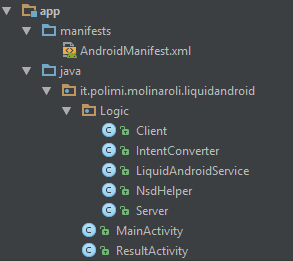
\includegraphics[width=.45\textwidth]{package}
	\caption{Code organization}
	\label{fig:5.1}
\end{figure}
As anticipated, the code is organized following the \textit{MVC} design pattern, so the \textit{controller components} are all contained in the \textit{Logic} package, while the \textit{UI components} are left inside the \textit{Main} package of the application- Other components typical of the Android development framework are left in their standard locations, such as the XML file containing the \textit{application manifest}.

\subsubsection{Implicit Intents to listen}
\begin{figure}[h]
	\centering
	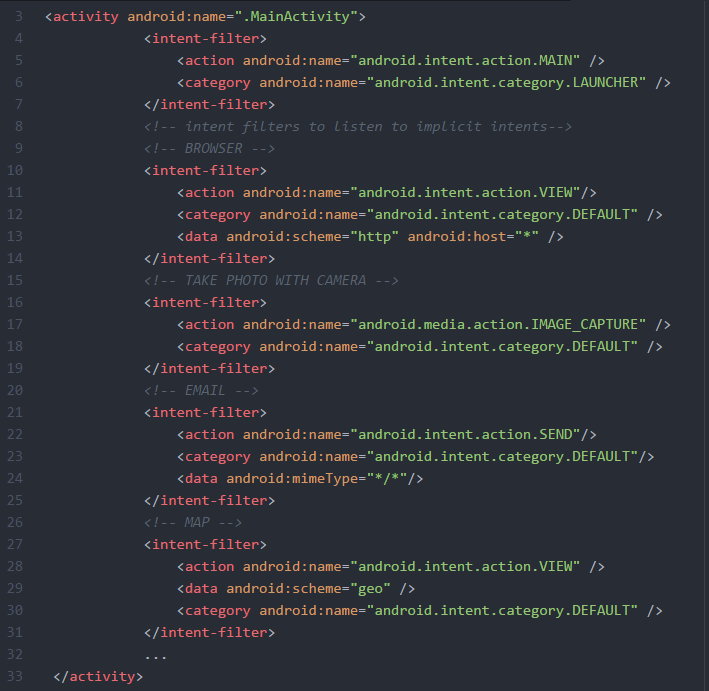
\includegraphics[width=.9\textwidth]{manifest}
	\caption{Liquid Android MainActivity Manifest}
	\label{fig:5.2}
\end{figure}
In \figurename~\ref{fig:5.2} there is part of the manifes, of my application, showing some common intent filter the \textit{Liquid Android} app can listen to. In figure we can see that is the MainActivity of the application which declare itself capable of managing intents to take a picture, send and email or open a map. By adding any intent filter to the manifest of the application Liquid Android can listen and forward, automatically any kind of Android implicit intent. This snippet of code is the way in which the \text{FR1} is practically implemented.\\\\
In the following section I want to describe my system in action, providing application's screenshots, UML diagrams, working tests and use cases.
\section{Working Demo}
blablablabla
\subsection{Live Test Cases}